\begin{frame}{Correct Proof}
    Assume that $f(A) = (1 - e^{-\frac{1}{2} + \delta})$
    \begin{center}
        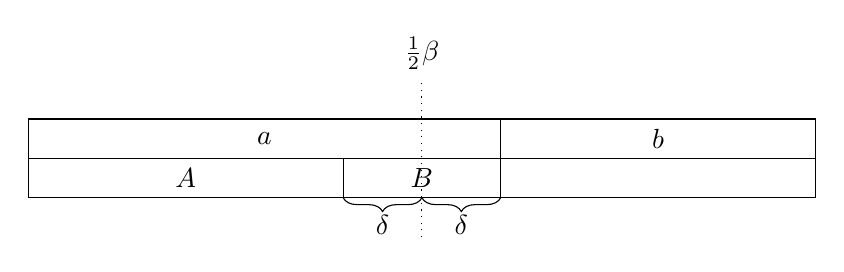
\begin{tikzpicture}
            \onslide<+(1)->{
                \draw (0,0)  rectangle (10, 1);
            }
            \onslide<+->{
                \draw[thin, dotted] (5, -.5) -- (5, 1.5) node[above, draw=none]{$\frac{1}{2}\beta$};
            }
            \only<+->{
                \draw[] (0,0) rectangle (4, .5) node[midway, draw=none]{$A$};
            }
            \only<+->{
                \draw (0, .5) rectangle (6, 1) node[midway, draw=none]{$a$};
            }
            \onslide<+->{
                \draw[decorate,decoration={brace,amplitude=5pt, mirror}]
                (4,0) -- (5,0) node[midway, below=1mm, draw=none]{$\delta$};
            }
            \only<+->{
                \draw[] (6, .5) rectangle (10, 1) node[draw=none, midway]{$b$};
            }
            \only<+->{
                \draw[decorate,decoration={brace,amplitude=5pt, mirror}]
                (5,0) -- (6,0) node[midway, below=1mm, draw=none]{$\delta$};
            }
            \only<+->{
                \draw (4, 0) rectangle (6, .5) node[draw=none, midway]{$B$};
            }
        \end{tikzpicture}
    \end{center}
    \onslide<+->{
    $$
    \begin{array}{ll}
        f(B|A) & \geq (1 - e^{-\frac{2\delta}{\frac{1}{2} - \delta}})f(O \setminus A \setminus a)
        \\
        & \geq (1 - e^{\frac{-2\delta}{\frac{1}{2} - \delta}})(f(O) - f(A) - f(a))
        \\
        & \vdots
        \\
        f(A \cup B) & \geq f(A) + f(B|A) \geq \dots \geq (1 + e^{-\frac{1}{2}})f(O)
    \end{array}
    $$
    }
\end{frame}